%% Standalone supplementary material (PROVISIONAL, evidence only): second 3-D implementation (FEniCSx) of the Hessenthaler Phase I model and a matched early-time cross-code comparison with a reconstruction of the solids4foam feature-edge protocol.
%% Build (from this directory):  latexmk -pdf supplement_fenicsx_hessenthaler.tex
%% It does not read article.aux. Data, scripts, provenance: paper-data/fenicsx_hessenthaler/ (README.md there).
\documentclass[sn-mathphys,Numbered]{sn-jnl}
\usepackage{graphicx}
\usepackage{amsmath,amssymb,amsfonts,bm}
\usepackage{xcolor}
\usepackage{soul}
\usepackage{manyfoot}
\usepackage{booktabs}
\usepackage{siunitx}
\usepackage{float}
\usepackage[utf8]{inputenc}
\usepackage[onehalfspacing]{setspace}
\usepackage[section]{placeins}
\usepackage{geometry}
\geometry{a4paper,textwidth=15cm,textheight=24cm}
\setlength{\parskip}{\baselineskip}
\renewcommand{\thesection}{S\arabic{section}}
\renewcommand{\thefigure}{S\arabic{figure}}
\renewcommand{\thetable}{S\arabic{table}}
\renewcommand{\theequation}{S\arabic{equation}}
\newcommand{\todo}[1]{\par\noindent\textcolor{red}{\rule{\linewidth}{0.8pt}}\par\nopagebreak
	\noindent{\small\color{red!70!black}\textbf{AUTHOR NOTE:} #1\par}\nopagebreak
	\noindent\textcolor{red}{\rule{\linewidth}{0.8pt}}\par}
\newcommand{\pending}[1]{\textcolor{red}{[\textbf{PENDING:}~#1]}}
% regenerated; do not edit
\newcommand{\matchedtable}{%
\begin{tabular}{rrrrrrrrr}\toprule
$t$ (s) & tip s4f & tip FE Gmi & diff (\%) & $F_y$ s4f & $F_y$ FE & $F_z$ s4f & $F_z$ FE & s4f its\\
& (mm) & (mm) & & ($\mu$N) & ($\mu$N) & ($\mu$N) & ($\mu$N) & \\ \midrule
0.10 & 0.0147 & 0.0157 & +6.7 & -112.7 & -111.1 & -553.1 & -580.8 & 4\\
0.20 & 0.1813 & 0.1794 & -1.0 & -346.4 & -340.8 & -708.2 & -746.2 & 4\\
0.30 & 0.8568 & 0.8220 & -4.1 & -573.3 & -560.4 & -630.0 & -659.9 & 4\\
0.40 & 2.3841 & 2.2650 & -5.0 & -710.0 & -691.1 & -536.1 & -533.4 & 4\\
0.50 & 4.3044 & 4.0981 & -4.8 & -700.3 & -712.4 & -310.5 & -283.6 & 5\\
0.60 & 4.8391 & 4.7990 & -0.8 & -324.7 & -377.5 & -425.2 & -448.7 & 4\\
0.70 & 11.2952 & 11.6230 & +2.9 & -70.2 & 229.8 & 981.7 & 848.1 & 5\\
0.75 & 14.9826 & 15.6428 & +4.4 & -791.9 & -756.8 & 1334.3 & 1208.1 & 3\\
\bottomrule\end{tabular}}
\newcommand{\tipstats}{mean -1.3\,\%, rms 3.8\,\%, maximum 6.7\,\% (37 common times, $0.1\le t\le0.75$\,s)}
\newcommand{\clstats}{rms 0.133\,mm, maximum 0.227\,mm (26 points)}

% regenerated; do not edit
\newcommand{\temporaltable}{%
\begin{tabular}{rrrrrrr}\toprule
$t$ (s) & tip s4f & tip Gc $\Delta t{=}0.005$ & tip Gc $\Delta t{=}0.02$ & $F_y$ s4f & $F_y$ Gc 0.005 & $F_y$ Gc 0.02\\
& (mm) & (mm) & (mm) & ($\mu$N) & ($\mu$N) & ($\mu$N) \\ \midrule
0.10 & 0.0147 & 0.0129 & 0.0155 & -112.7 & -109.7 & -109.2\\
0.30 & 0.8568 & 0.7986 & 0.8179 & -573.3 & -546.3 & -548.1\\
0.50 & 4.3044 & 4.0573 & 4.0327 & -700.3 & -743.8 & -718.1\\
0.60 & 4.8391 & 4.5498 & 4.7980 & -324.7 & -454.6 & -399.1\\
0.62 & 5.5684 & 5.2624 & 5.4780 & -61.2 & -263.0 & -230.2\\
0.64 & 6.7679 & 6.5011 & 6.6300 & 319.4 & 82.4 & -18.4\\
0.66 & 8.2523 & 8.1085 & 8.1977 & 556.9 & 413.3 & 175.2\\
0.70 & 11.2952 & 11.4392 & -- & -70.2 & 69.0 & --\\
0.75 & 14.9826 & 15.3042 & 15.9086 & -791.9 & -986.9 & -745.0\\
\bottomrule\end{tabular}}

\newcommand{\data}{\detokenize{paper-data/fenicsx_hessenthaler}}

\begin{document}

\title[Supplementary material: FEniCSx Hessenthaler Phase I]{Supplementary material (provisional): a second three-dimensional implementation (FEniCSx) of the Hessenthaler Phase I benchmark and a matched early-time comparison with a solids4foam feature-edge reconstruction}

\author*[1]{\fnm{Author} \sur{Placeholder}}\email{corresponding.author@example.org}
\affil[1]{\orgdiv{School of Mechanical and Materials Engineering}, \orgname{University College Dublin}, \orgaddress{\country{Ireland}}}

\maketitle

\todo{PROVISIONAL, EVIDENCE ONLY. This is not a completed Hessenthaler verification and not an MRI validation. No settled solution exists in either code; the corrected feature-edge reference runs of the main text (feF1--feF3) were not available when this was written, and the solids4foam results below are OUR reconstruction of the protocol described in the Hessenthaler section of the main text, not the author's runs. Same research group, same AI model lineage: neither a second group nor an independent verification.}

\section{Purpose and status}
The aim is a cross-code consistency check of the three-dimensional Phase~I model over the time interval that both codes could be run on the corrected (feature-edge) geometry at an affordable cost: the first $0.75\,\mathrm{s}$, i.e.\ the $0.5\,\mathrm{s}$ inflow/buoyancy ramp and $0.25\,\mathrm{s}$ after it. Three things are reported: (i) the model and a FEniCSx implementation with standalone checks (Sections~\ref{sec:model}--\ref{sec:checks}); (ii) a matched-physical-time comparison of tip displacement, interface force and deformed centreline with solids4foam (Section~\ref{sec:matched}); (iii) what is missing and what failed (Section~\ref{sec:limits}). Nothing here changes the classification of the benchmark, and agreement in an early transient is not evidence of convergence or of accuracy at the steady state.

\section{Model and equivalence}\label{sec:model}
Fixed model, identical in both codes by construction or by source reading: published fluid surface with $250\,\mathrm{mm}$ outlet extension; flap $11\times2\times65\,\mathrm{mm}$ clamped at $z=0$, flow along $+z$; $\rho_F=1163.3$, $\nu_F=1.0745\times10^{-5}$, $\rho_S=1058.3$; compressible neo-Hookean solid $W=\tfrac{\mu}{2}(\bar I_1-3)+\tfrac{K}{4}(J^2-1-2\ln J)$ with $\mu=64.2\,\mathrm{kPa}$, $\nu=0.45$ ($K=620.6\,\mathrm{kPa}$), shown equal to the solids4foam law (\texttt{517a44921}, source lines 213--222: $\bm\sigma=\mu J^{-1}\mathrm{dev}(\bar{\bm b})+\tfrac K2 (J^2-1)J^{-1}\bm I$); net buoyancy $(\rho_S-\rho_F)\bm g/\rho_S=0.973306\,\mathrm{m/s^2}$ along $+y$, ramped with the inflow by $3s^2-2s^3$ over $0.5\,\mathrm{s}$; parabolic inlets $630$ and $615\,\mathrm{mm/s}$; fixed outlet pressure with the backflow-stabilised traction $\bm\sigma\bm n=\beta\rho_F\min(\bm u\cdot\bm n,0)\bm u$, $\beta=0.2$. $\mu$ was not changed to improve any agreement.
\begin{table}[htbp]\centering\caption{Differences between the two computations (they limit what the comparison can show).}\label{tab:diff}\small
\begin{tabular}{@{}p{2.9cm}p{5.2cm}p{5.5cm}@{}}\toprule
 & FEniCSx (this work) & solids4foam (reconstruction, ours)\\\midrule
discretisation & monolithic ALE, P2/P1/P2 tetrahedra, one conforming mesh & partitioned IQN-ILS, cell-centred FV fluid ($236\,114$ cells), cell-centred solid S2 ($6\,240$ hexahedra, stabilisation 0.01), AMI transfer\\
convection & Galerkin & LUST, unlimited least-squares gradients\\
time step & $0.02\,\mathrm{s}$ ($0.01\,\mathrm{s}$ for $t>0.69\,\mathrm{s}$), BDF2 & $0.002\,\mathrm{s}$, BDF2\\
geometry & wall decimated from the published surface (max.\ deviation $0.12\,\mathrm{mm}$), flap exact & published surface meshed directly, feature edges captured\\
resolution & Gmi: $118\,278$ tets, flap faces $1.22\,\mathrm{mm}$ & feF1-like: flap $0.505\,\mathrm{mm}$\\
coupling test & Newton to $10^{-8}$ & strict test (both measures $<10^{-4}$), 3--11 coupling iterations\\
mesh motion & harmonic extension of the total displacement & velocity Laplacian\\\bottomrule
\end{tabular}\end{table}

\section{FEniCSx implementation}\label{sec:fenicsx}
Unknowns $(\bm u,p,\bm d)$ on one tetrahedral mesh (fluid and flap cells, shared interface): $\bm u$ P2, $p$ P1, $\bm d$ P2; fluid in ALE form in the reference configuration, conservative discrete GCL, BDF2 with variable step; solid total-Lagrangian; the interface traction is the natural sum of the fluid and solid momentum residuals (exact Nanson measure); $\bm d$ in the fluid solves a harmonic extension. Newton (PETSc SNES, exact UFL Jacobian) with a linear-extrapolation predictor for the initial guess, GMRES preconditioned by a block Gauss--Seidel of solid+interface (LU), ALE (GAMG) and fluid (LU) blocks, or by a global MUMPS LU that is reused across Newton iterations; same equations in all variants. Source, solver options and versions: \texttt{\data/README.md}. Verified by independent means: the discrete momentum identities of the assembled equations hold to $4\times10^{-11}\,\mu\mathrm N$ ($I-f_b=R_{BC}+W_{\rm all}$ on three states, Section~\ref{sec:checks}); the Jacobian agrees with finite differences ($10^{-15}$--$10^{-9}$ in $u$ and $p$, second-order in the displacement directions); the converged states are identical with the global LU and with the block preconditioner.

\section{Geometry and mesh}
The published surface (sha256 of the file in the solids4foam tutorial: \texttt{0be13c04\ldots}) is a $123\,156$-triangle anisotropic CAD triangulation; its wall patch was decimated (quadric, max.\ deviation $0.12\,\mathrm{mm}$, area $+0.004\,\%$) and inlets, outlet, the exact flap box and the clamp rectangle were rebuilt, so that fluid and solid share the same interface triangles (checked: every interface triangle has one fluid and one solid cell; flap area error $<10^{-8}$; solid volume error $10^{-8}$). Preregistered gate (minimum SICN $>0.05$, inlet areas within $0.5\,\%$): passed by Gmi ($118\,278$ tets) and G0 ($198\,658$); the coarser level Gc fails the inlet-area criterion ($0.9\,\%$) and is used only for development and sensitivity (marked ``dev''). The solids4foam reconstruction mesh (cfMesh with \texttt{surfaceFeatureEdges -angle 45}, level ``coarse'') has $236\,114$ cells (main-text table: $233\,956$, $+0.9\,\%$), maximum non-orthogonality $61.65^\circ$ (table: $61.6^\circ$), interface area $1711.97\,\mathrm{mm^2}$ (exact $1712$).

\section{Standalone checks}\label{sec:checks}
\textbf{Material law.} Analytic against automatic differentiation $2\times10^{-15}$, consistent tangent against finite differences $5\times10^{-10}$, frame indifference $10^{-14}$ (all preregistered thresholds passed).
\textbf{Zero-flow flap, $\mu=64.2$\,kPa.} P2 tetrahedra, three nested solid meshes: tip $28.992$, $29.257$, $29.338\,\mathrm{mm}$, monotone, observed order $1.70$, Richardson $29.374\,\mathrm{mm}$ (conditional, three levels). The preregistered prediction interval $[29.20,29.60]$ was met. As a diagnostic only, the modulus that would give the measured $29.50\,\mathrm{mm}$ is $62.6$ and $63.4\,\mathrm{kPa}$ on the first two levels and about $63.8\,\mathrm{kPa}$ in the limit (two-point interpolation in $\mu$, conditional Richardson), against the calibration limit $63.95\,\mathrm{kPa}$ (GCI $0.42$) already in the main text: a preliminary second-implementation check of the law and boundary conditions, of the order of $0.2\,\%$; it is not used to select the modulus.
\textbf{Fluid only, flap held fixed (Gmi, ramp to $0.5\,\mathrm{s}$).} Mass imbalance $4\times10^{-10}$, inflow within $0.05\,\%$ of nominal, no backflow, Newton $\le4$.
\textbf{Interface force definitions.} On three states the force on the flap was reconstructed independently from the assembled residuals (variationally consistent nodal force, with and without the clamp-constrained nodes) and from the facet traction integral. The identities above close to $10^{-11}\,\mu\mathrm N$: there is no action--reaction defect. The facet traction differs from the nodal force of the free nodes by $3.5$--$6\,\%$ at the clamped root edge; the thin flap's net lateral load is a small difference of large face pressures ($\approx7$\,mN per face against $\approx0.1$\,mN), which is why interface-load definitions matter in this benchmark.

\section{Matched early-time comparison}\label{sec:matched}
Only identical physical times are compared. The solids4foam run (ours, case files and log extract in \texttt{\data/s4f\_case/}, \texttt{logs/}) follows the main-text protocol for the feature-edge campaign with the deltas listed in \texttt{prereg/ADDENDUM\_A6b.md} (written before the run); it ran strictly converged from $t=0$ ($3$--$11$ coupling iterations per step, both residual measures below $10^{-4}$ at every step (largest $9.98\times10^{-5}$), no step accepted unconverged, continuity error $10^{-13}$). The flap tip is the point $(0,0,65\,\mathrm{mm})$ in both codes; the force on the flap is the solids4foam ``solid interface'' total, and for FEniCSx the facet traction integral.
\begin{table}[htbp]\centering\caption{Matched physical times. Tip $y$ displacement and force components on the flap (fluid acting on the flap). FE Gmi: dt $0.02\,\mathrm{s}$ ($0.01\,\mathrm{s}$ from $0.69\,\mathrm{s}$); s4f: dt $0.002\,\mathrm{s}$, our reconstruction.}\label{tab:matched}\scriptsize\setlength{\tabcolsep}{3pt}\matchedtable\end{table}
Over the common times the tip differs by \tipstats; the deformed centreline at $t=0.69\,\mathrm{s}$ differs by \clstats\ (Figure~\ref{fig:cl}). Both codes show the same shape of the transient: a slow rise during the ramp, a plateau of the tip near $4.3$--$4.8\,\mathrm{mm}$ at $0.5$--$0.6\,\mathrm{s}$ and a rapid rise afterwards (tip $\approx15\,\mathrm{mm}$ at $0.75\,\mathrm{s}$), and a reversal of the axial force near $0.63$--$0.64\,\mathrm{s}$ (Figures~\ref{fig:tip}, \ref{fig:forces}). The lateral force $F_y$ agrees to within $3\,\%$ up to $0.5\,\mathrm{s}$ (Gmi, $\Delta t=0.02\,\mathrm{s}$) and the axial force $F_z$ to within $9\,\%$ up to $0.6\,\mathrm{s}$ but only to $14\,\%$ at $0.7\,\mathrm{s}$; the sharp peak of $F_y$ near $0.66\,\mathrm{s}$ is present in both codes but on the accepted level it is about a factor two lower than in solids4foam and changes sign later (e.g.\ $F_y=-70$ against $+230\,\mu$N at $0.7\,\mathrm{s}$) (Table~\ref{tab:matched}, Figure~\ref{fig:forces}) and is the least reliable quantity here (temporal sensitivity, see below). Differences are classified, not tuned away: resolution (Gmi flap faces $1.22\,\mathrm{mm}$ against $0.505\,\mathrm{mm}$), time step, convection scheme, coupling (monolithic against partitioned), interface transfer and force definition (s4f ``fluid'' and ``solid'' interface totals differ by $3.5\,\%$ in $F_y$ at $0.1\,\mathrm{s}$; the FEniCSx facet and nodal forces differ by $4$--$6\,\%$), outlet treatment, wall decimation. One resolution per code does not support a continuum or mesh-convergence statement. \paragraph{Temporal control (development level).} Because the FEniCSx step ($0.02\,\mathrm{s}$) is ten times the solids4foam step, the Gc level was rerun from $t=0$ with $\Delta t=0.005\,\mathrm{s}$ (same mesh and numerics, preregistered question and criterion in \texttt{prereg/ADDENDUM\_A7.md}). The tip changes by at most 7.0\,\% (rms 3.1\,\%) for $t\ge0.2\,\mathrm{s}$ (and by 17\,\% at $t=0.1\,\mathrm{s}$, where the tip is micrometres), and the peak of $F_y$ near $0.67\,\mathrm{s}$ rises from 237 to 472\,$\mu$N, against 563\,$\mu$N in solids4foam (72\,\% of the gap closed): (sample maxima: the $\Delta t=0.02\,\mathrm{s}$ peak is under-sampled, so this fraction is uncertain); on the accepted level Gmi the sample maximum of $F_y$ is only 290\,$\mu$N at $t=0.69\,\mathrm{s}$, about half of the solids4foam peak, and $F_y$ has the opposite sign at $0.7\,\mathrm{s}$ (Table~\ref{tab:matched}). The height of the $F_y$ peak is therefore largely a time-step effect in the FEniCSx data at $\Delta t=0.02\,\mathrm{s}$ (shown on the development level only), and the tip agreement of Table~\ref{tab:matched} contains temporal errors of the same order as the differences it reports (at $\Delta t=0.005\,\mathrm{s}$ the development-level tip is $-6\,\%$ below solids4foam at $0.6\,\mathrm{s}$ and $+2\,\%$ above at $0.75\,\mathrm{s}$). This is one mesh and two time steps: it is neither a temporal convergence study nor an error bound. The step used in Table~\ref{tab:matched} was not changed to improve agreement.\par\begin{table}[htbp]\centering\caption{Temporal control on the development level Gc (not an accepted level) against solids4foam (ours).}\label{tab:temporal}\scriptsize\setlength{\tabcolsep}{3pt}\temporaltable\end{table}

\begin{figure}[H]\centering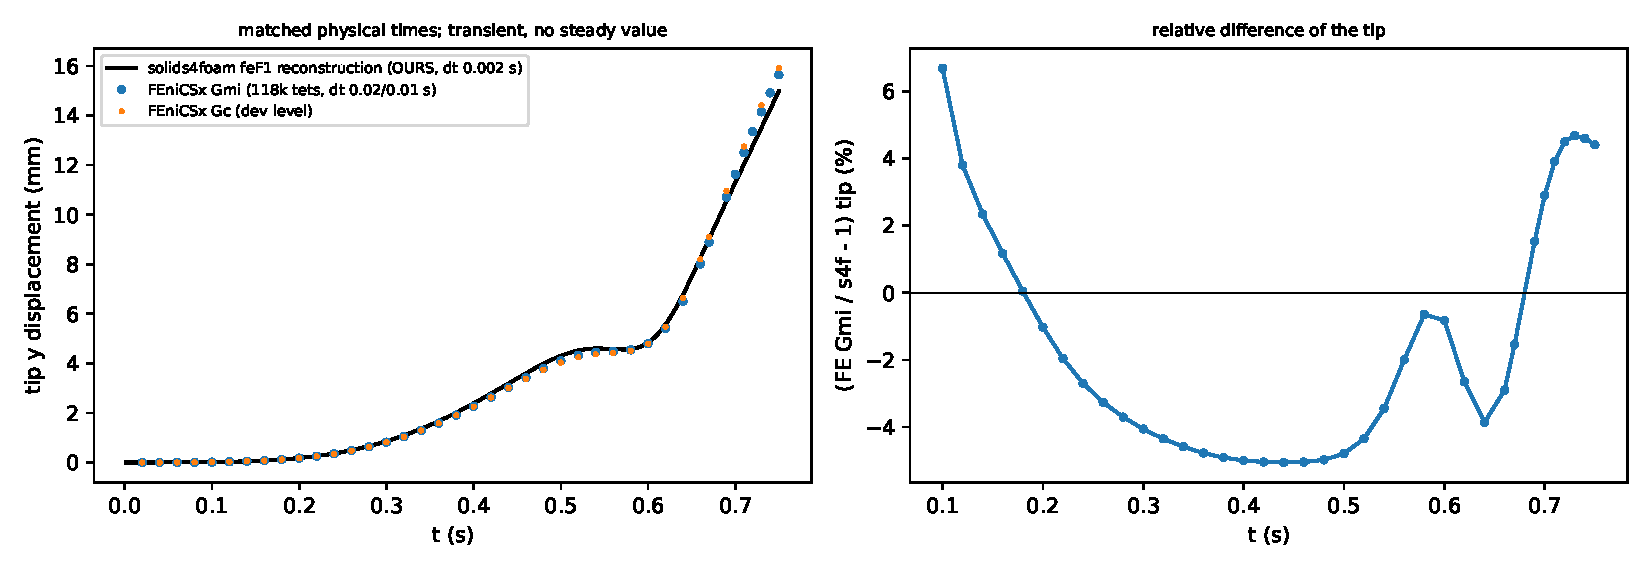
\includegraphics[width=\textwidth]{paper-data/fenicsx_hessenthaler/figures/fig_tip_matched.pdf}\caption{Tip displacement at matched times (left) and relative difference (right). Transient only: no steady value is implied.}\label{fig:tip}\end{figure}
\begin{figure}[H]\centering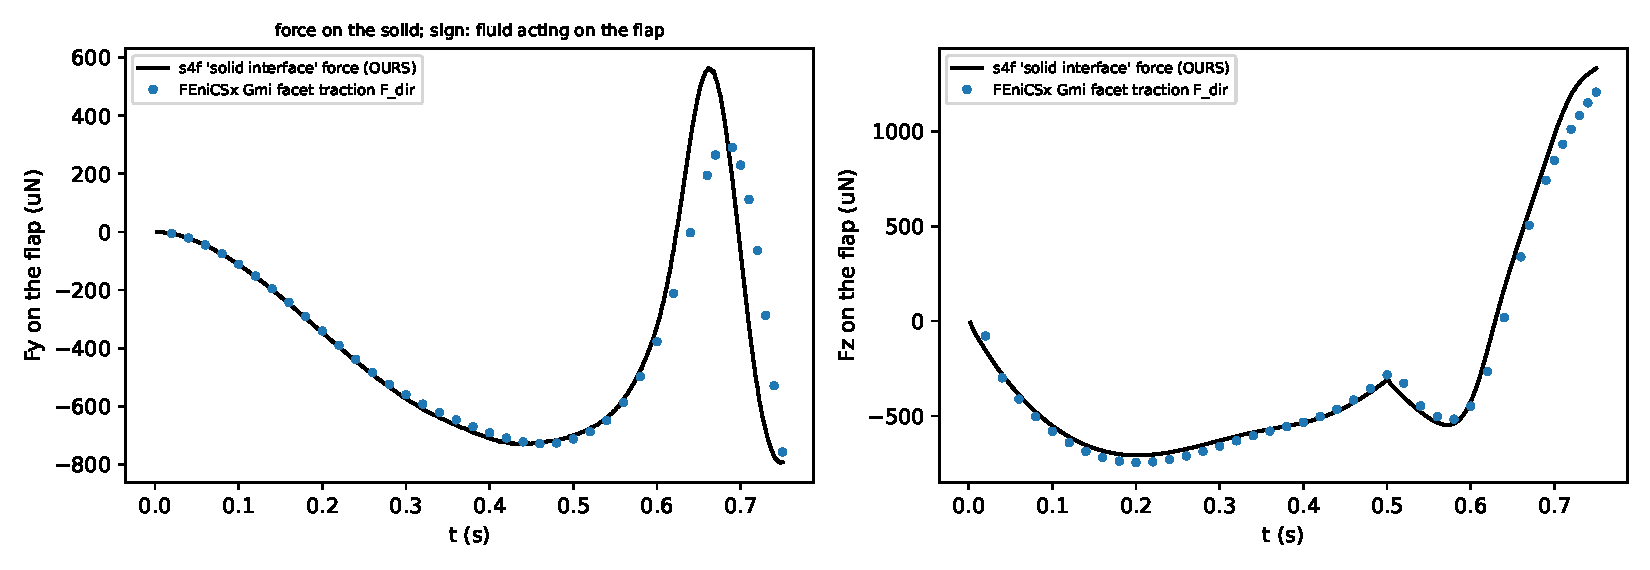
\includegraphics[width=\textwidth]{paper-data/fenicsx_hessenthaler/figures/fig_forces_matched.pdf}\caption{Force components on the flap at matched times.}\label{fig:forces}\end{figure}
\begin{figure}[H]\centering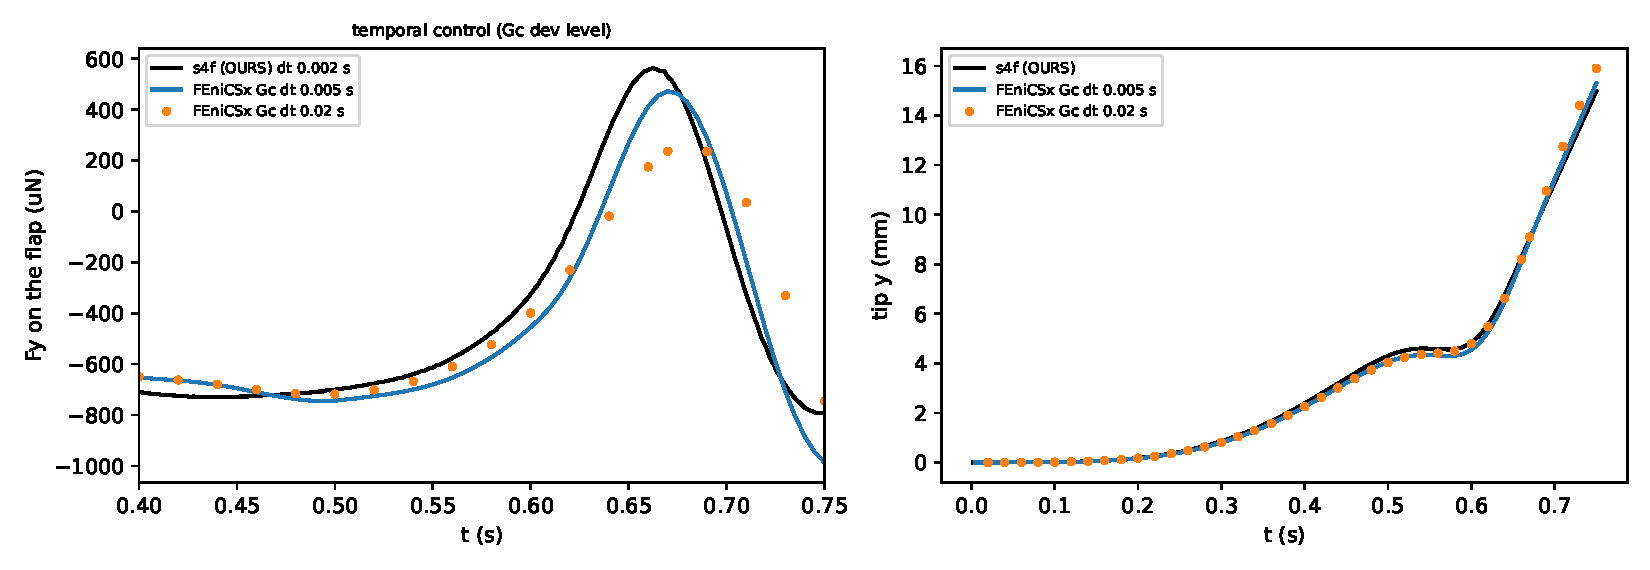
\includegraphics[width=\textwidth]{paper-data/fenicsx_hessenthaler/figures/fig_temporal_control.pdf}\caption{Temporal control on the development level Gc: $F_y$ (left, zoom) and tip (right) for $\Delta t=0.02$ and $0.005\,\mathrm{s}$ against solids4foam.}\label{fig:temporal}\end{figure}
\begin{figure}[H]\centering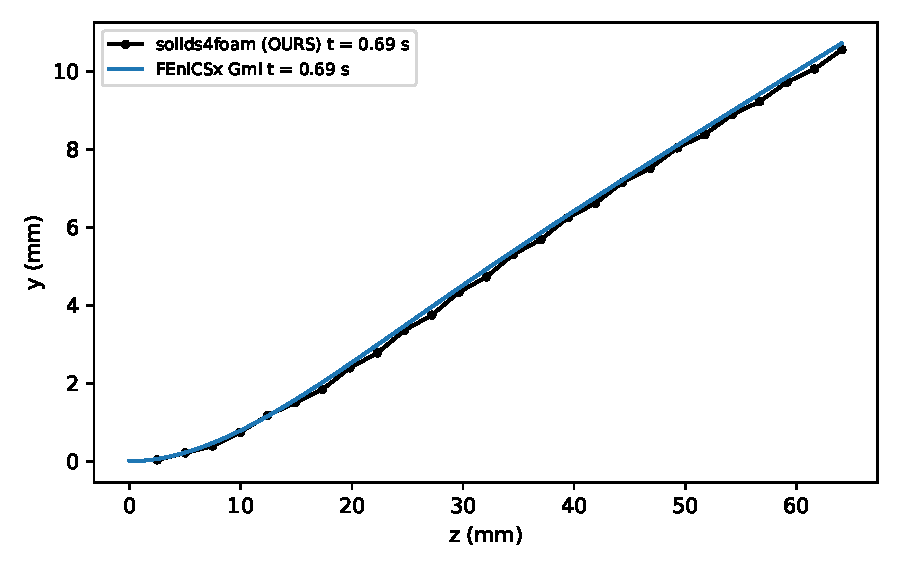
\includegraphics[width=0.62\textwidth]{paper-data/fenicsx_hessenthaler/figures/fig_centreline_0p69.pdf}\caption{Deformed centreline at $t=0.69\,\mathrm{s}$ ($x=0$).}\label{fig:cl}\end{figure}

\section{What is missing, what failed}\label{sec:limits}
\begin{itemize}
\item The corrected feF1--feF3 results of the main text were unavailable; the solids4foam numbers are our reconstruction (equivalence with the author's runs is unverified: our mesh has $0.9\,\%$ more cells, and the solver source differs from the unpublished verification branch).
\item No settled state in either code; the FEniCSx solution exists to $0.75\,\mathrm{s}$ on the accepted level and to $1.21\,\mathrm{s}$ on the development level; beyond $\approx0.76\,\mathrm{s}$ the accepted-level fluid mesh deteriorates (minimum ALE $\det F=0.2$ gate). The steady tip, the MRI centreline and the MRI velocities are not compared; the MRI data are validation data and no uncertainty is available.
\item One FEniCSx accepted level (Gmi); a third spatial level could not be generated; no order, no GCI, no Richardson value for the coupled problem.
\item Solver development failed in part: fieldsplit/GAMG, ASM-ILU, selfp Schur and LSC preconditioners for the fluid block did not reach a true residual of $10^{-6}$ (preserved, \texttt{runs} listed in the README); the working configurations need a direct factorisation (cost: about $1.3$--$2.9$ CPU-h per step on Gmi, $19.3$ CPU-h per simulated second for the solids4foam reconstruction on 16 cores).
\item Interface-force definitions differ by $3.5$--$6\,\%$ between facet traction and nodal force at the root; the literal registered facet-based balance criterion was not met, the identity-based balance was.
\end{itemize}

\section{Reproducibility}
Raw histories, the fixed case files of both codes, hashes (\texttt{SHA256SUMS}), the preregistration addenda with their hashes (written before the corresponding runs), versions and commands: \texttt{\data/README.md} and \texttt{SOURCES.md}. Tables and figures are regenerated from the CSV files by \texttt{scripts/}.

\end{document}
